% =====================================================================
%  c02 —— PDF p.17–25（原书 p.11–19）
%  §1.4–§1.6
%  块首承接：原书 p.10 末段延续到 p.11 的部分（Definition 1.4 两条的讨论）
%  已由 c01 译完，本块从 p.11 的「例（分类叠）」起译。
% =====================================================================

% ===== 原书 p.11 =====
\noindent\textbf{例（分类叠）.}
$X$为代数簇，$G$为作用在$X$上的有限群。此时令叠$[X/G]$为以如下(1)、(2)构成的组$(\tilde Y\to Y,\tilde Y\to X)$为对象的范畴：
\begin{enumerate}[label=(\arabic*)]
\item $\tilde Y\to Y$是$G$-齐性空间，
\item $\tilde Y\to X$是$G$-等变态射。
\end{enumerate}
此时，把对象$(\tilde Y\to Y,\tilde Y\to X)$对应到$Y$的函子$[X/G]\to(\Sch/\C)$是代数叠。实际上可以证明$X\to[X/G]$是平展满射。

\subsection{Algebraic stack $\MbarG$ 及其性质}

所论的$\MbarG$是代数叠，只需验证下面的 M.Artin 判别法，这一点已知。

\begin{theorem}[M.Artin]
满足以下两个条件的叠$S\to\Sch(k)$是代数的。
\begin{enumerate}[label=(\arabic*)]
\item $S\to S\times_{\Sch(k)}S$可表且非分歧。
\item 存在由$k$上有限型概形给出的可表叠$X$，以及从$X$出发的光滑满射态射$f:X\to S$。
\end{enumerate}
% ===== 原书 p.12 =====
这里，态射$f$光滑，是指对任意概形$Y$与任意$Y\to S$，基变换$X\times_SY$可表，且$X\times_SY\to Y$光滑。
\end{theorem}

证明此处不给出。实际来验证这些条件成立。

\noindent\textbf{条件(1).}
$S\to S\times_{\Sch(k)}S$可表，是指：对任意态射$X\to S\times_{\Sch(k)}S$，把对应的稳定曲线记为$C_1\to X$、$C_2\to X$时，由对角映射拉回所得的概形由$\Isom_X(C_1,C_2)$表示。只要说明它实际上在$X$上非分歧即可。概形间态射非分歧，可用下面这个无穷小的等价说法。

\begin{lemma}
概形的态射$f:X\to Y$非分歧（resp.\ 光滑），当且仅当对$k$的任意扩域$L$与交换图
\[
\begin{tikzcd}
X(\Spec L[\epsilon]/\epsilon^2) \arrow[r, "f_1"] \arrow[d, "p_X"'] & Y(\Spec L[\epsilon]/\epsilon^2) \arrow[d, "p_Y"] \\
X(\Spec L) \arrow[r, "f_0"'] & Y(\Spec L)
\end{tikzcd}
\]
下述条件成立：对满足$f_0(x)=p_Y(y)$的$x\in X(\Spec L)$与$y\in Y(\Spec L[\epsilon]/\epsilon^2)$，满足$p_X(z)=x$、$f_1(z)=y$的$z\in X(\Spec L[\epsilon]/\epsilon^2)$至多有一个（resp.\ 必定存在）。
\end{lemma}

把这个非分歧判别法用到态射$\Isom_X(C_1,C_2)\to X$上。$\Isom_X(C_1,C_2)\to X$非分歧，只需对$L[\epsilon]/\epsilon^2$上的稳定曲线$C\to\Spec(L[\epsilon]/\epsilon^2)$，说明$\Aut(C)\to\Aut(C\times\Spec(L))$是单射。令$C\times\Spec(L)=C_0$，则这个核作为群同构于$\Hom_{\mathcal{O}_{C_0}}(\omega_{C_0},\mathcal{O}_{C_0})$。计算结果是$0$。因此$\Isom_X(C_1,C_2)\to X$非分歧。

\noindent\textbf{条件(2).}
只要说明取$H_g$作为条件中的$X$即可。现设从可表叠$X$到$\MbarG$的态射$f:X\to\MbarG$已给出，对应的稳定曲线为$C\to X$，则$H_g\times_{\MbarG}X\to X$由$\Isom_X(\mathbf{P}^{5g-6},\operatorname{Proj}(f_*(\omega_{C/X}^{\otimes3})))$给出。$f_*(\omega_{C/X}^{\otimes3})$是$X$上的向量丛，因此$H_g\times_{\MbarG}X\to X$是$X$上的光滑满射。

% ===== 原书 p.13 =====
下面说明$\MbarG$的光滑性与紧合性。

\begin{definition}[分离性（separatedness）、紧合性（properness）、光滑性（smoothness）]
设$S\to\Sch(k)$为代数叠。
\begin{enumerate}[label=(\arabic*)]
\item $S\to\Sch(k)$分离，是指对角态射$S\to S\times_{\Sch(k)}S$紧合。
\item 分离代数叠$S\to\Sch(k)$紧合，是指存在$k$上紧合的可表叠$X\to\Sch(k)$与$\Sch(k)$上的满射态射$X\to S$。
\item 代数叠$S\to\Sch(k)$光滑，是指存在由光滑概形表示的叠$X$与平展满射态射$X\to S$。
\end{enumerate}
\end{definition}

\transnote{原文定义 1.5 标题印作「separetedness, propoerness, smoothness」，前两词有拼写错误，此处按「分离性、紧合性、光滑性」译出。}

这里想提醒一点：即使$S$作为代数叠光滑，对应的解析空间$S(\C)$一般也不光滑。实际上，正如下文所述，$\MbarG$作为代数叠光滑，但对应的解析空间$\MbarG(\C)$具有称为商奇点（quotient singularity）的奇点。

\begin{theorem}[Deligne--Mumford {[DM]}]
$\MbarG$是紧合光滑代数叠。
\end{theorem}

下面使用如下引理。

\begin{lemma}[valuative criterion]
$\Sch(k)$上分离的代数叠$S\to\Sch(k)$若满足以下条件，则紧合。设$V$为离散赋值环，$K$为其分式域，给定交换图
\[
\begin{tikzcd}
\Spec(K) \arrow[r] \arrow[d] & S \arrow[d] \\
\Spec(V) \arrow[r] & \Sch(k)
\end{tikzcd}
\]
% ===== 原书 p.14 =====
则存在$V$上有限的离散赋值环$V'$与态射$\Spec(V')\to S$，使下面的交换图存在：
\[
\begin{tikzcd}
\Spec(K') \arrow[r] \arrow[d] & \Spec(V') \arrow[d] \\
\Spec(K) \arrow[r] & S
\end{tikzcd}
\]
\end{lemma}

\begin{proof}
略。
\end{proof}

\noindent\textbf{证明定理 1.6.}
先说明分离性。换言之，给定概形$X$与稳定曲线$C_1\to X$、$C_2\to X$，要说明态射$\Isom_X(C_1,C_2)\to X$紧合。由赋值判别法，这归结为说明以下事实。
\begin{quote}
给定离散赋值环$V$上的稳定曲线$C_1,C_2$，以及它们的一般纤维$C_{1K}$、$C_{2K}$之间的$K$-同构$\phi_K:C_{1K}\to C_{2K}$，此时$\phi_K$唯一地延拓为$C_1,C_2$的同构$\phi:C_1\to C_2$。
\end{quote}
一般地，给定离散赋值域$K$上的曲线$C_K$时，若$V$上的稳定曲线$C$以$C_K$为一般纤维，则称$C$为$C_K$在$V$上的稳定模型（stable model）。$K$上的曲线若存在稳定模型，则除同构外唯一；这一事实正是分离性的另一种说法。它本质上由曲面论中（相对）极小模型的唯一性得到证明。（详见 Deligne--Mumford [DM]。）

承认分离性后，要证紧合性可用引理 1.7。即只需证明下面的定理。

\begin{theorem}[stable reduction theorem]
设$K,V$如上，给定$K$上的曲线$C_K$。此时存在$V$上有限的赋值环$V'$与其上的稳定曲线$C'$，令$K'$为$V'$的分式域，则$C'$到$K'$的限制$C'_{K'}$与$C_K$到$K'$的基变换一致。
\end{theorem}

\begin{proof}[证明概略]
$K$上的曲线$C_K$是$V$上半稳定曲线的一般纤维时，称$C$为$C_K$的半稳定模型（semi-stable model）。若$C_K\ne\emptyset$，则由 Raynaud 可知，相对 Picard 概形$\Pic^0(C)$是$\Pic^0(C_K)$的 Néron 模型。

% ===== 原书 p.15 =====
设$l$为与$V$的剩余特征互素的素数。由 Grothendieck 关于 abelian variety 的半稳定归约定理，$l$-进表示$T_l(\Pic^0(C_K))$幂零，这等价于$\Pic^0(C_K)$的 Néron 模型$\Pic^0(C)$的特殊纤维没有幂幺根（unipotent radical）。另一方面，$\Pic^0(C)_s$是$C_s$的 Picard 群，因此计算$\Pic^0(C_s)=H^1(C_s,\mathcal{O}^\times)$可知，它没有幂幺根，这等价于$C_s$是既约正规交叉。进一步用 Artin--Lipman 定理，把$(-1)$-曲线、$(-2)$-曲线吹落，便可构造$V$上的半稳定曲线$\tilde C$。综合这些可知，$l$-进表示$T_l(\Pic^0(C_k))$是幂幺的，这等价于$C_K$具有半稳定模型。又$T_l(\Pic^0(C_k))$限制到$\operatorname{Gal}(\bar K/K)$的充分小的有限指数子群上时幂零，故得到定理 1.8。
\end{proof}

\transnote{原文此处两处将 $C_K$ 写作 $C_k$，疑为笔误，译文照原文保留 $C_k$。}

以上证明了$\MbarG$是紧合光滑代数叠。

\subsection{Algebraic stack 的上同调理论}

设$S$为$\Spec(\C)$上紧合光滑的代数叠。此时如下定义$H^*(S,\mathbf{Q})$。

首先取可表的$X$与平展满射$\varphi:X\to S$。此时令$S$上$(n+1)$个纤维积为$X_n=X\times_S\cdots\times_SX$，它是由光滑概形表示的叠。在其上考虑按解析流形拓扑理解的$\mathbf{R}\Gamma(X_n,\mathbf{Q})$。这里$\mathbf{R}\Gamma(X_n,\mathbf{Q})$虽由导出范畴定义，但把它理解为$X_n$的奇异上链复形
\[
0\to C^0(X_n,\mathbf{Q})\to C^1(X_n,\mathbf{Q})\to\cdots
\]
即可。导出范畴中，若两个复形之间存在拟同构，即在同调意义下引起同构的复形态射，就把这两个复形视为同一。$\mathbf{R}\Gamma(X_n,\mathbf{Q})\otimes\C$还有另一个代表（原文称为实现，realization），即 de Rham 复形
\[
0\to A^0(X_n)\to A^1(X_n)\to\cdots
\]
现在，对$i=0,\ldots,n+1$，定义$\pi_{n+1,i}:X_{n+1}\to X_n$为
\[
(x_0,\ldots,x_{n+1})\mapsto(x_0,\ldots,\hat x_i,\ldots,x_{n+1}),
\]
由此诱导的映射记作$\pi^*_{n+1,i}:\mathbf{R}\Gamma(X_n,\mathbf{Q})\to\mathbf{R}\Gamma(X_{n+1},\mathbf{Q})$。进一步定义

% ===== 原书 p.16 =====
$\delta:\mathbf{R}\Gamma(X_n,\mathbf{Q})\to\mathbf{R}\Gamma(X_{n+1},\mathbf{Q})$为$\delta(x)=\sum_{i=0}^{n+1}(-1)^i\pi^*_{n+1,i}(x)$，便得到双复形
\[
0\to\mathbf{R}\Gamma(X_0,\mathbf{Q})\to\mathbf{R}\Gamma(X_1,\mathbf{Q})\to\mathbf{R}\Gamma(X_2,\mathbf{Q})\to\cdots
\]
把这个双复形的伴随单复形（associated simple complex）记作$s(\mathbf{R}\Gamma(X_\bullet,\mathbf{Q}))$。

% 原书在此处出现 Proposition 1.8 与 Theorem 1.8 重号（原书自身如此），
% 按导言区说明单点复现该编号。
\addtocounter{theorem}{-1}
\begin{proposition}
设$X,Y$为概形，$\varphi:X\to S$、$\psi:Y\to S$为平展满射态射，则$s(\mathbf{R}\Gamma(X_\bullet,\mathbf{Q}))$与$s(\mathbf{R}\Gamma(Y_\bullet,\mathbf{Q}))$拟同构。
\end{proposition}

\transnote{原书第 16 页的命题 1.8 与第 14 页的定理 1.8 重号，此为原书自身如此，译本在此处照原书编号复现。}

由命题 1.8，把$s(\mathbf{R}\Gamma(X_\bullet,\mathbf{Q}))$的拟同构类记作$\mathbf{R}\Gamma(S,\mathbf{Q})$。为强调是在经典拓扑下考虑，也写作$\mathbf{R}\Gamma(S_{\mathrm{an}},\mathbf{Q})$。

\begin{proof}
使用上同调下降（cohomology descent）的方法。现取两个代数簇$V,W$与平展满射态射$\varphi:V\to W$，把$V$在$W$上的$(i+1)$个纤维积$V\times_W\cdots\times_WV$记作$V_i$。与前面定义的一样，可定义双复形
\[
0\to\mathbf{R}\Gamma(V_0,\mathbf{Q})\to\mathbf{R}\Gamma(V_1,\mathbf{Q})\to\cdots
\]
把它的伴随单复形记作$s(\mathbf{R}\Gamma(V_\bullet,\mathbf{Q}))$，则自然映射$\mathbf{R}\Gamma(W,\mathbf{Q})\to s(\mathbf{R}\Gamma(V_\bullet,\mathbf{Q}))$由下降理论可知是拟同构。

据此考虑下面的双单纯概形$X_\bullet\times_SY_\bullet$。
\begin{center}
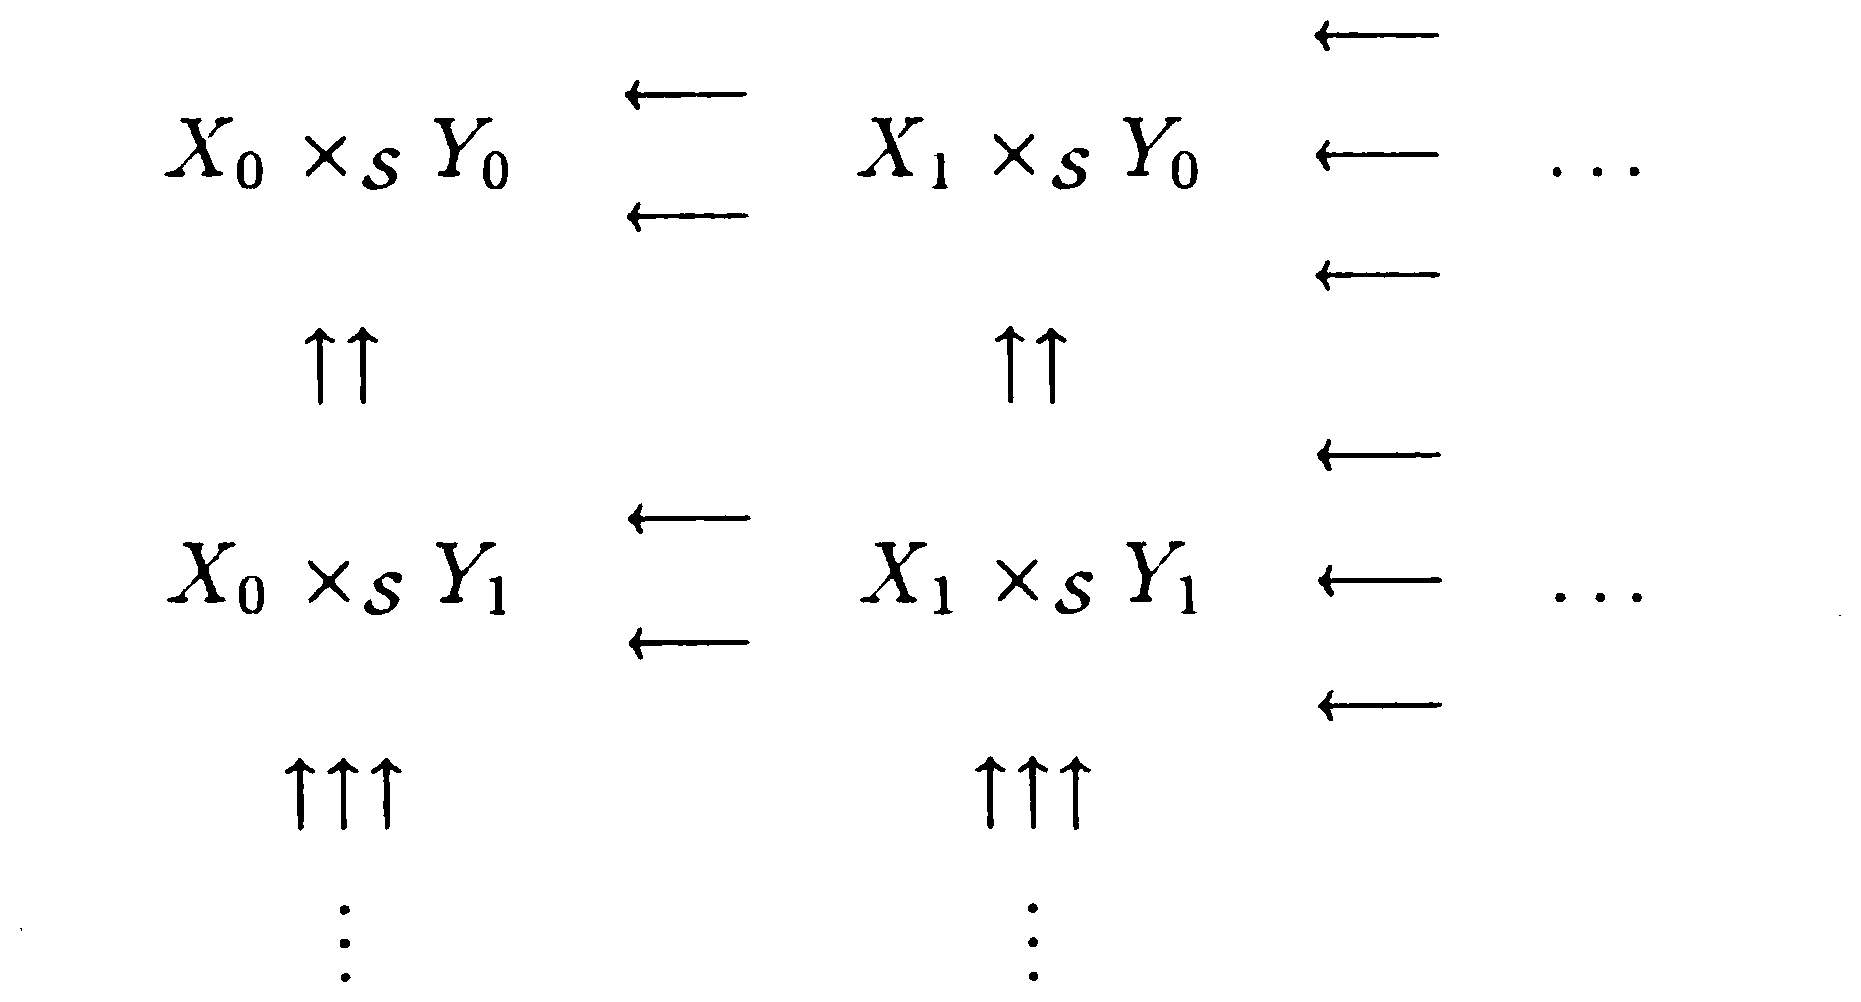
\includegraphics[width=0.62\linewidth]{fig_p22_a.png}
\end{center}
此时，由前面的注，
\[
X_i\times_SY_j=(X_i\times_SY_0)\times_{X_i}\cdots\times_{X_i}(X_i\times_SY_0)\qquad((j+1)\text{ 个})
\]
注意到这一点，便有$\mathbf{R}\Gamma(X_i,\mathbf{Q})\cong s(\mathbf{R}\Gamma(X_i\times Y_\bullet,\mathbf{Q}))$。

% ===== 原书 p.17 =====
因此$s(\mathbf{R}\Gamma(X_\bullet,\mathbf{Q}))\cong s(\mathbf{R}\Gamma(X_\bullet\times Y_\bullet,\mathbf{Q}))$。这里右边是双单纯概形的伴随单复形。另一方面，右边关于$X$与$Y$对称，故得到$s(\mathbf{R}\Gamma(X_\bullet\times Y_\bullet,\mathbf{Q}))\cong s(\mathbf{R}\Gamma(Y_\bullet,\mathbf{Q}))$。
\end{proof}

奇异同调也如下定义。令$C_\bullet(X,\mathbf{Q})$为$X$的$\mathbf{Q}$系数奇异同调。由此得到双复形
\[
\to C_\bullet(X_2,\mathbf{Q})\to C_\bullet(X_1,\mathbf{Q})\to C_\bullet(X_0,\mathbf{Q})
\]
把它的伴随单复形记作$C_\bullet(S,\mathbf{Q})$。其第$i$同调记作$H_i(S,\mathbf{Q})$。取 de Rham 实现（realization），便由积分得到自然的配对$H_i(S,\mathbf{Q})\otimes H^i(S,\mathbf{Q})\to\C$。

\transnote{原文把 $C_\bullet(X,\mathbf{Q})$ 称为「$X$ 的 $\mathbf{Q}$ 系数奇异同调」；严格说 $C_\bullet$ 是奇异链复形，其同调才是 $H_i$。译文照原文保留，此处仅作说明。}

其次定义迹映射。$S$为$\Spec(\C)$上紧合不可约代数叠时，存在与$S$同维的紧合不可约概形$X$与满射$\pi:X\to S$。把$\pi$的次数$\deg(X/S)$定义为：对支配态射$\varphi:Y\to S$，$\pi$的基变换$Y\times_SX\to Y$的次数；它是良定义的。把$X$的迹映射$\tr_X:H^{2d}(X,\mathbf{Q})\to\mathbf{Q}$（$d=\dim X$）与自然映射$\pi^*:H^{2d}(S,\mathbf{Q})\to H^{2d}(X,\mathbf{Q})$组合，令$\tr_S=(\deg(X/S))^{-1}\tr_X\circ\pi^*$，便定义迹映射$\tr_S$。它不依赖于$\pi:X\to S$的取法，这一点再由纤维积的讨论可知。

\subsection{$n$ 点稳定曲线的模理论}

Knudsen--Mumford 作为 Deligne--Mumford 结果的精密化，证明了$n$点稳定曲线的模问题可由代数叠表示。设$C,S$为基础域$k$上的有限型概形，$f:C\to S$与$n$个截面$s_1,\ldots,s_n:S\to C$是亏格$g$的稳定曲线，是指满足以下条件(1)--(5)。

\begin{enumerate}[label=(\arabic*)]
\item $f$在$S$上紧合平坦，相对维数为$1$。
\item 对各$s\in S$，纤维$f^{-1}(s)$既约，且至多只有通常二重点。
% ===== 原书 p.18 =====
\item $\dim H^1(f^{-1}(s),\mathcal{O}_{f^{-1}(s)})=g$。
\item $s_i(s)$包含在$f^{-1}(s)$的光滑点中。
\item $f^{-1}(s)$的有理分支包含$3$个以上的点，这些点是截面像$s_i(s)$或与其它分支的交点。
\end{enumerate}

令$\MbarGN$为亏格$g$的$n$点稳定曲线$(f:C\to S,s_1,\ldots,s_n)$的范畴，令$\MbarGN\to\Spec(k)$为把上述数据对应到$S$的函子，则它是代数叠。与前面一样，对概形$X$，给出$X\to\MbarGN$与给出亏格$g$的$n$点稳定曲线$(f:C\to X,s_1,\ldots,s_n)$等价。现在给定$(n+1)$点稳定曲线$(f:C\to S,s_1,\ldots,s_{n+1})$时，忘掉$s_{n+1}$，考虑$n$个截面$s_1,\ldots,s_n$。此时$(f:C\to S,s_1,\ldots,s_n)$一般不是$n$点稳定曲线；但考虑集合
\[
\begin{aligned}
\{s\in S\mid{}&\text{在 }f^{-1}(s)\text{ 中 }s_{n+1}\text{ 落在某个有理分支 }C_i\text{ 内，}\\
&\text{且 }C_i\text{ 只含 }s_i(s)\text{ 与其它分支的交点这 }3\text{ 个点}\},
\end{aligned}
\]
它定出$S$的闭子簇$Z$。设$C_i$为$f^{-1}(Z)$内与$C_i$对应的$\mathbf{P}^1$-丛（实际上，由于被$3$个点标记，它与$f^{-1}(Z)\times\mathbf{P}^1$同型）。此时$C_i\subset C$可以吹落，把结果所得的曲线记作$\bar f:\bar C\to S$。这时$(\bar f:\bar C\to S,s_1,\ldots,s_n)$是$n$点稳定曲线。$S$特别是一维且$C$光滑时，下面两个是典型的例子。

\begin{center}
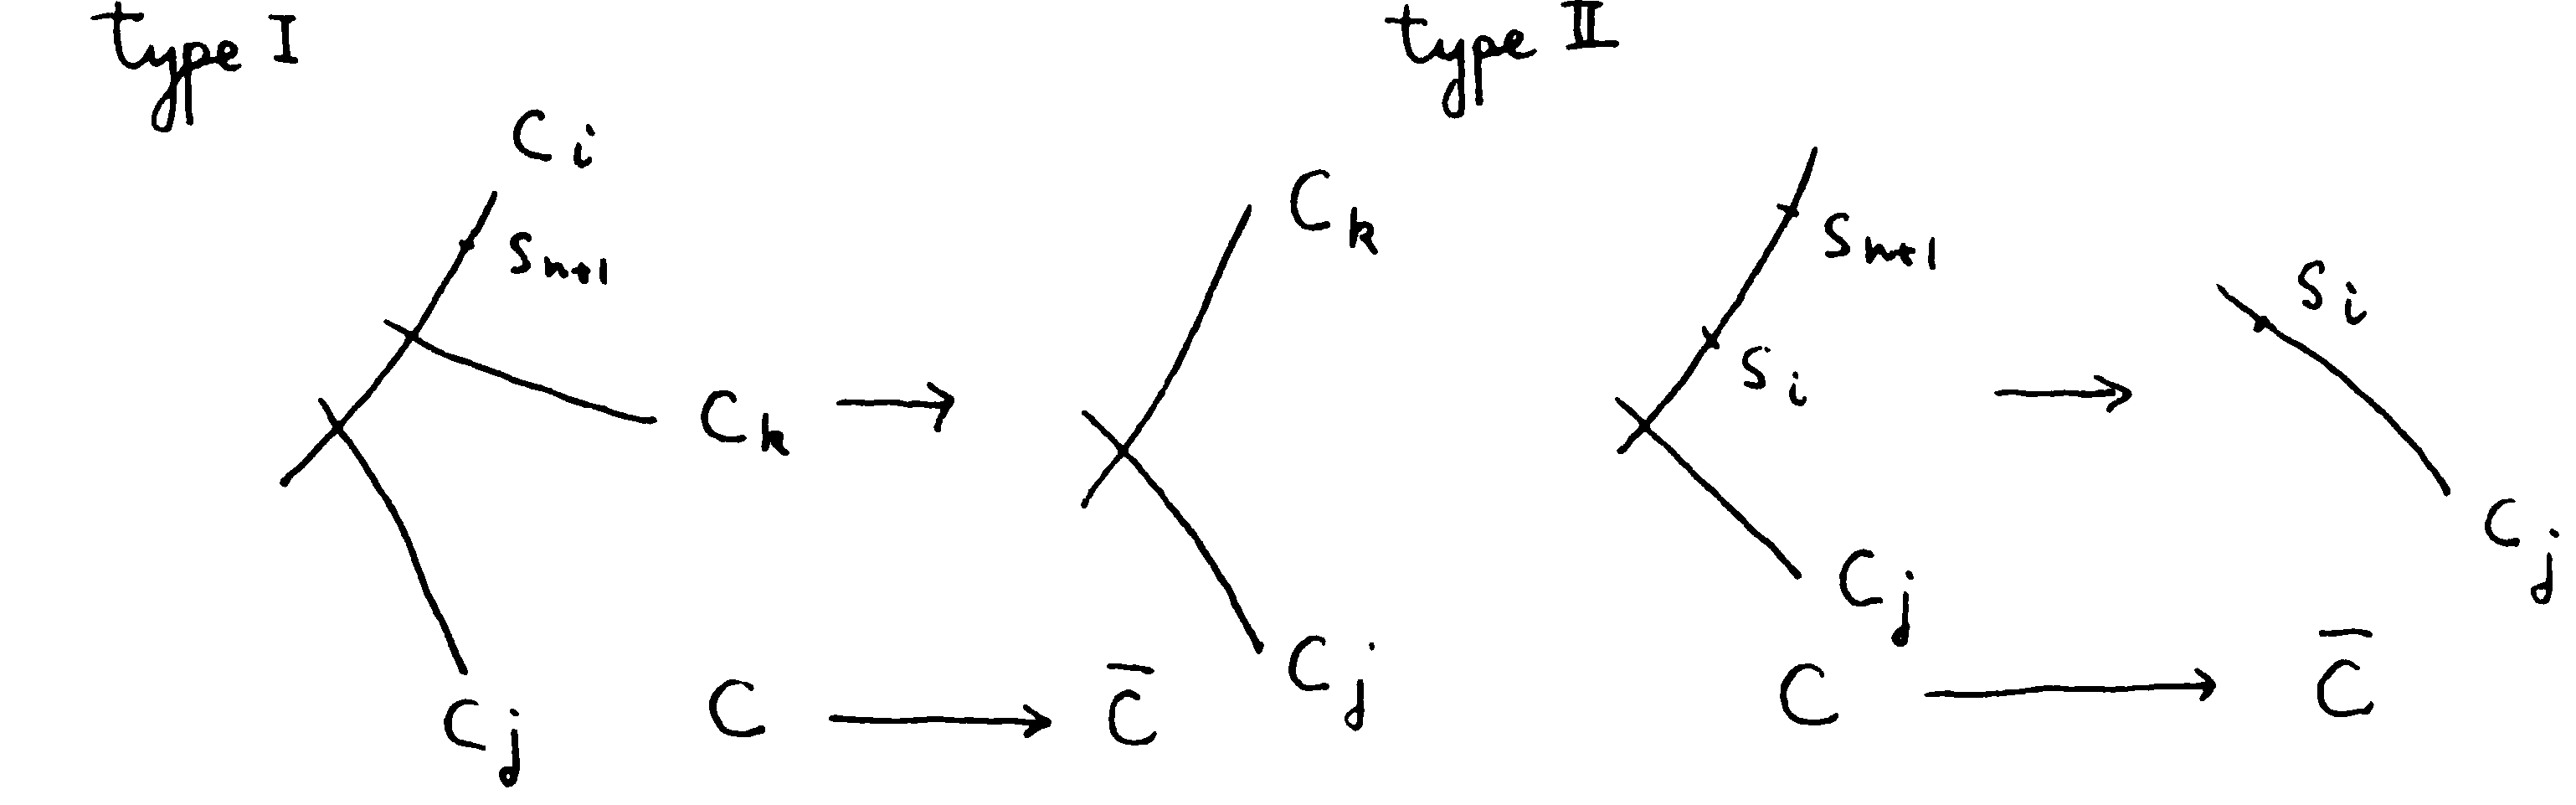
\includegraphics[width=0.9\linewidth]{fig_p24_a.png}
\end{center}

由此得到函子$\MbarN{g,n+1}\to\MbarGN$。

\begin{theorem}[Knudsen--Mumford {[KM]}]
\begin{enumerate}[label=(\arabic*)]
\item 现给定$X\to\MbarGN$，即给定亏格$g$的$n$点稳定曲线$(f:C\to X,s_1,\ldots,s_n)$。此时
% ===== 原书 p.19 =====
$C$自然同构于$\MbarN{g,n+1}\times_{\MbarGN}X$，$f$经此同构与第二投影$\MbarN{g,n+1}\times_{\MbarGN}X\to X$等同（视为同一）。
\item $\MbarGN$是紧合光滑代数叠。
\end{enumerate}
\end{theorem}

由(1)的性质，称$\MbarN{g,n+1}\to\MbarGN$为万有曲线。特别地，$\MbarN{g,1}\to\MbarG$是$\MbarG$上的万有曲线。其次构造万有截面$\tilde s_i:\MbarGN\to\MbarN{g,n+1}$（$i=1,\ldots,n$）。对$\MbarGN$的对象$(f:C\to X,s_1,\ldots,s_n)$，$s_i(X)$是$C$的除子。沿它在$X\times\mathbf{P}^1$内把除子$X\times\{0\}$粘到$C$上，把所得对象记作$\tilde C$。再定义两个截面$s'_i,s_{n+1}:X\to\tilde C$，分别由$X\to X\times\{1\}$、$X\to X\times\{\infty\}$给出。此时$(\tilde f:\tilde C\to X,s_1,\ldots,s'_i,\ldots,s_n,s_{n+1})$是$(n+1)$点稳定曲线。由此得到万有截面$\tilde s_i:\MbarGN\to\MbarN{g,n+1}$。

\begin{center}
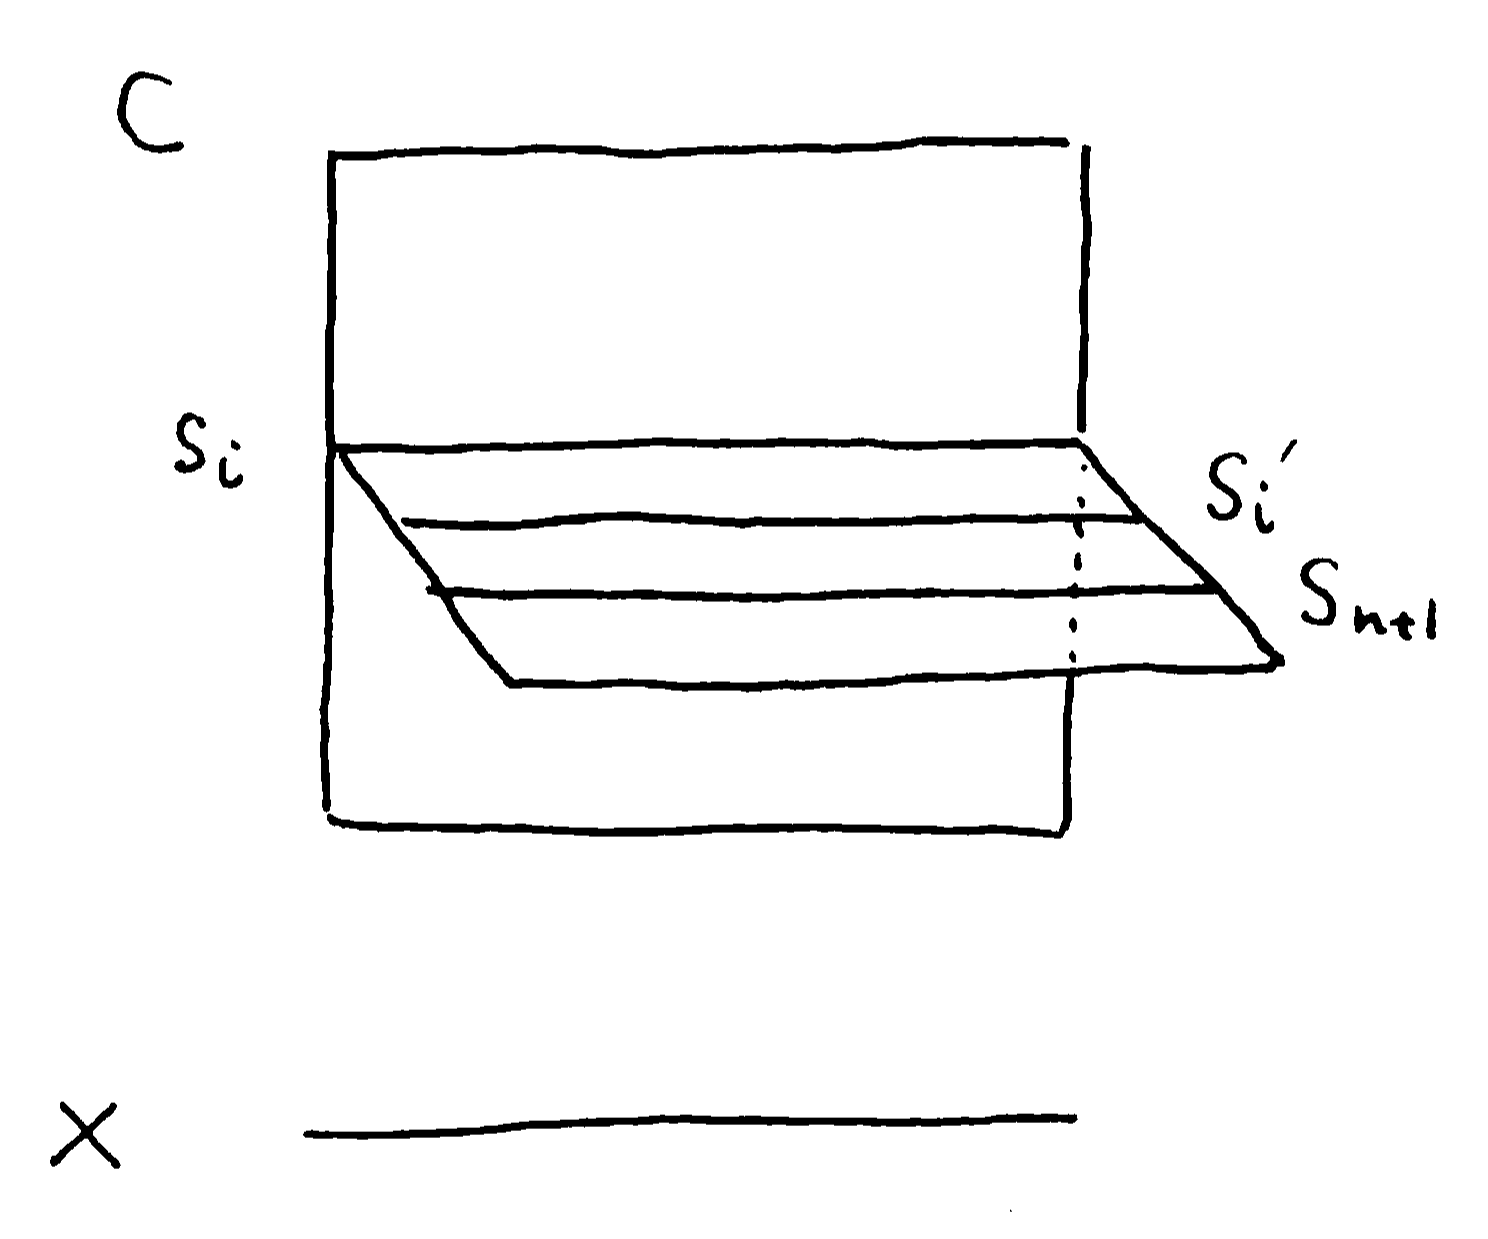
\includegraphics[width=0.55\linewidth]{fig_p25_a.png}
\end{center}
